
%----------------------------------------------------------------------------------------
%	PACKAGES AND OTHER DOCUMENT CONFIGURATIONS
%---------------------------------------------------------------------------------------

\documentclass[11pt]{scrartcl} % Font size
\newcommand{\comment}[1]{}
%%%%%%%%%%%%%%%%%%%%%%%%%%%%%%%%%%%%%%%%%
% Wenneker Assignment
% Structure Specification File
% Version 2.0 (12/1/2019)
%
% This template originates from:
% http://www.LaTeXTemplates.com
%
% Authors:
% Vel (vel@LaTeXTemplates.com)
% Frits Wenneker
%
% License:
% CC BY-NC-SA 3.0 (http://creativecommons.org/licenses/by-nc-sa/3.0/)
% 
%%%%%%%%%%%%%%%%%%%%%%%%%%%%%%%%%%%%%%%%%

%----------------------------------------------------------------------------------------
%	PACKAGES AND OTHER DOCUMENT CONFIGURATIONS
%----------------------------------------------------------------------------------------

\usepackage{amsmath, amsfonts, amsthm} % Math packages

\usepackage{listings} % Code listings, with syntax highlighting

\usepackage[english]{babel} % English language hyphenation

\usepackage{graphicx} % Required for inserting images
\graphicspath{{Figures/}{./}} % Specifies where to look for included images (trailing slash required)

\usepackage{booktabs} % Required for better horizontal rules in tables

\numberwithin{equation}{section} % Number equations within sections (i.e. 1.1, 1.2, 2.1, 2.2 instead of 1, 2, 3, 4)
\numberwithin{figure}{section} % Number figures within sections (i.e. 1.1, 1.2, 2.1, 2.2 instead of 1, 2, 3, 4)
\numberwithin{table}{section} % Number tables within sections (i.e. 1.1, 1.2, 2.1, 2.2 instead of 1, 2, 3, 4)

\setlength\parindent{0pt} % Removes all indentation from paragraphs

\usepackage{enumitem} % Required for list customisation
\setlist{noitemsep} % No spacing between list items

%----------------------------------------------------------------------------------------
%	DOCUMENT MARGINS
%----------------------------------------------------------------------------------------

\usepackage{geometry} % Required for adjusting page dimensions and margins

\geometry{
	paper=a4paper, % Paper size, change to letterpaper for US letter size
	top=2.5cm, % Top margin
	bottom=3cm, % Bottom margin
	left=3cm, % Left margin
	right=3cm, % Right margin
	headheight=0.75cm, % Header height
	footskip=1.5cm, % Space from the bottom margin to the baseline of the footer
	headsep=0.75cm, % Space from the top margin to the baseline of the header
	%showframe, % Uncomment to show how the type block is set on the page
}

%----------------------------------------------------------------------------------------
%	FONTS
%----------------------------------------------------------------------------------------

\usepackage[utf8]{inputenc} % Required for inputting international characters
\usepackage[T1]{fontenc} % Use 8-bit encoding

\usepackage{fourier} % Use the Adobe Utopia font for the document

%----------------------------------------------------------------------------------------
%	SECTION TITLES
%----------------------------------------------------------------------------------------

\usepackage{sectsty} % Allows customising section commands

\sectionfont{\vspace{6pt}\centering\normalfont\scshape} % \section{} styling
\subsectionfont{\normalfont\bfseries} % \subsection{} styling
\subsubsectionfont{\normalfont\itshape} % \subsubsection{} styling
\paragraphfont{\normalfont\scshape} % \paragraph{} styling

%----------------------------------------------------------------------------------------
%	HEADERS AND FOOTERS
%----------------------------------------------------------------------------------------

\usepackage{scrlayer-scrpage} % Required for customising headers and footers

\ohead*{} % Right header
\ihead*{} % Left header
\chead*{} % Centre header

\ofoot*{} % Right footer
\ifoot*{} % Left footer
\cfoot*{\pagemark} % Centre footer
 % Include the file specifying the document structure and custom commands
%\usepackage{flafter}
\usepackage[section]{placeins}
\usepackage{caption}
\usepackage{float}
%----------------------------------------------------------------------------------------
%	TITLE SECTION
%----------------------------------------------------------------------------------------

\title{	
	\normalfont\normalsize
	\textsc{Rutgers University, New Brunswick}\\ % Your university, school and/or department name(s)
	\vspace{25pt} % Whitespace
	\rule{\linewidth}{0.5pt}\\ % Thin top horizontal rule
	\vspace{20pt} % Whitespace
	{\huge CS 520 Final}\\ % The assignment title
	\vspace{12pt} % Whitespace
	\rule{\linewidth}{2pt}\\ % Thick bottom horizontal rule
	\vspace{12pt} % Whitespace
}

\author{\LARGE Eshaan Gandhi} % Your name

\date{\normalsize\today} % Today's date (\today) or a custom date

\begin{document}

\maketitle % Print the title
\section{Question 1}
\subsection{How many possible sheep/dog configurations might the field be in?}
This can be calculated using some combinatorial theory. We first select 3 blocks/squares from the grid. This can be done in 49 choose 3 ways, or like computer scientists would say binomial(49, 3). This equals 18424. Now of these 3 squares we need to choose 2 to put the dog in. This can be done is 3 choose 2 or binomial(3, 2) ways. This equals 3. Hence, the total configurations of the board are 18424*3 = 55272 ways to arrange the board or 55272 configurations possible. 
\subsection{For a given field configuration C(position of dogs, position of sheep), formulate a mathematical description for T(C), the minimal number expected rounds needed to corner the sheep. Hint:  For what configurations C is T(C) easy to compute?} 
The way I thought about this was a recurrence problem. The easiest configurations to be solve are the ones where the sheep is pinned to one of the four walls and one where the dogs are on top and on the left of the sheep.\\
By setting up like this we can see that the base case of "dogs are on top and on the left of the sheep" needs $12-m-n$ steps before the sheep is pinned. In this way we have certain configurations that we already know the answer to. I thought it would be beneficial to then try to reach this configuration. \\
The expression I came up with is this
\begin{center}
$T(C) = \sum \frac{1}{\#\ of\ possible\ sheep\ moves}*(1+T_{x1, x2, s}(C))$
\end{center} 
The new configuration is calculated by averaging out all the states that the sheep can be in. For example, if the sheep is open to move in all four directions then
\begin{center}
$T(C) = 1/4(1+T_{x1, x2, (s[0], s[1]+1)}C)+1/4(1+T_{x1, x2, (s[0]+1, s[1])}C)+1/4(1+T_{x1, x2, (s[0], s[1]-1)}C)+1/4(1+T_{x1, x2, (s[0]-1, s[1])}C)$
\end{center}
Notice the sheep moves right, down, left, and up. Now as far as the x1 and x2 are concerned, they are coordinates of the two dogs. The dogs are trying to get into the position. I run a BFS search to find the most optimal dog to choose to try and chase the squares. 

\subsection{If you could calculate T(C) for any configuration C, show that you could construct an optimal dog-controlling algorithm for cornering the sheep.}
If there is a T(C) for any configuration C, there is a fixed number of steps you need to take in order to corner the sheep in the \textbf{minimum} number of rounds. Since you can do this in the minimum number of rounds there has to be a deterministic approach to solve this maze for any configuration. Since there is a deterministic way to approach this problem, we can construct an optimal dog-controlling algorithm for cornering the sheep. 

\subsection{Write an algorithm and code to solve for the function T.  Is T always finite?  What does it mean when T is infinite?}
The code I wrote works under the assumption that since the movements are completely random, it gives us a good enough idea of the sheep's location when the dog gets there. The above formula would work but is very complex and memory heavy, and python cannot handle it. Functional programming languages can do a better job at that. Hence my code uses a simplified version to give us a basic heuristic of what the number of rounds required can be. I used the relaxation that the sheep on average would be in it's own square and the dogs can run to round it. \\
The agent works in the following way
\begin{itemize}
\item The dogs first try to round the top and left squares of the sheep. This helps them round it in the least amount of time. If this is possible then the sheep is rounded is 12-m-n rounds. Where m and n are the x and y coordinates of the sheep. 
\item Then they try to pin the sheep in the bottom left or top right corner and drag it along the boundaries. This pins the sheep in 12-m or 12-n depending on the boundary, after the dogs have arrived. 
\item The last case is when the sheep is unfortunately pinned in the top left corner of the grid. This makes the dogs do the most work as they have to drag the sheep through the boundaries.  
\end{itemize}
The function Tc is the relaxation version while T is the actual recursive model.\\
T seems to be always finite since number of configurations of the board is finite. All of the configurations on the board have a solution. Since every configuration can be broken down into constituent configuration, till the base case is reached, T is always finite. 

\subsection{Given the initial configuration in the above example, how many rounds do you need (on average) to corner the sheep?}
It takes 18 rounds on average to corner the sheep. 
\subsection{What is the worst possible initial state (position of dog bots, sheep), and why? Justify mathematically.}
The worst initial state for the dog bots and the sheep is going to be when the sheep is in the top left corner and the dog bots are in the bottom right corner. This can be seen as the dogs would have to do the most work to get to the top right corner and then the most work to get the sheep down to bottom right. This makes us explore more configurations, and each configuration increases the number of rounds it takes to corner the sheep. 
\subsection{You are allowed to place your dog bots anywhere in the field at the start, then the sheep will be placed uniformly
at random in one of the remaining unoccupied cells. Where should you place your dog bots initially, and why?
Justify mathematically.}
The dog should be placed in the top left corners as this removes the chance of the sheep being placed there. This also allows us to reach the best state of the dog bots being on the top and left as easily as possible. 
\subsection{Do you think better strategies exist than the one you came up with? Justify.}
I don't think better a better strategy exists as BFS path is the shortest and the most optimal path to get to a square and there is no faster and deterministic way to solve it without those base cases. \\
\paragraph{Note}
Thinking I came up with the best strategy possible is a bit narcissistic. 
\section{Question 2 - Bot Negotiations}
\subsection{The State Transition Diagram}
This is the state transition diagram that helped me solve this markov decision process. 
\begin{figure}[H]
  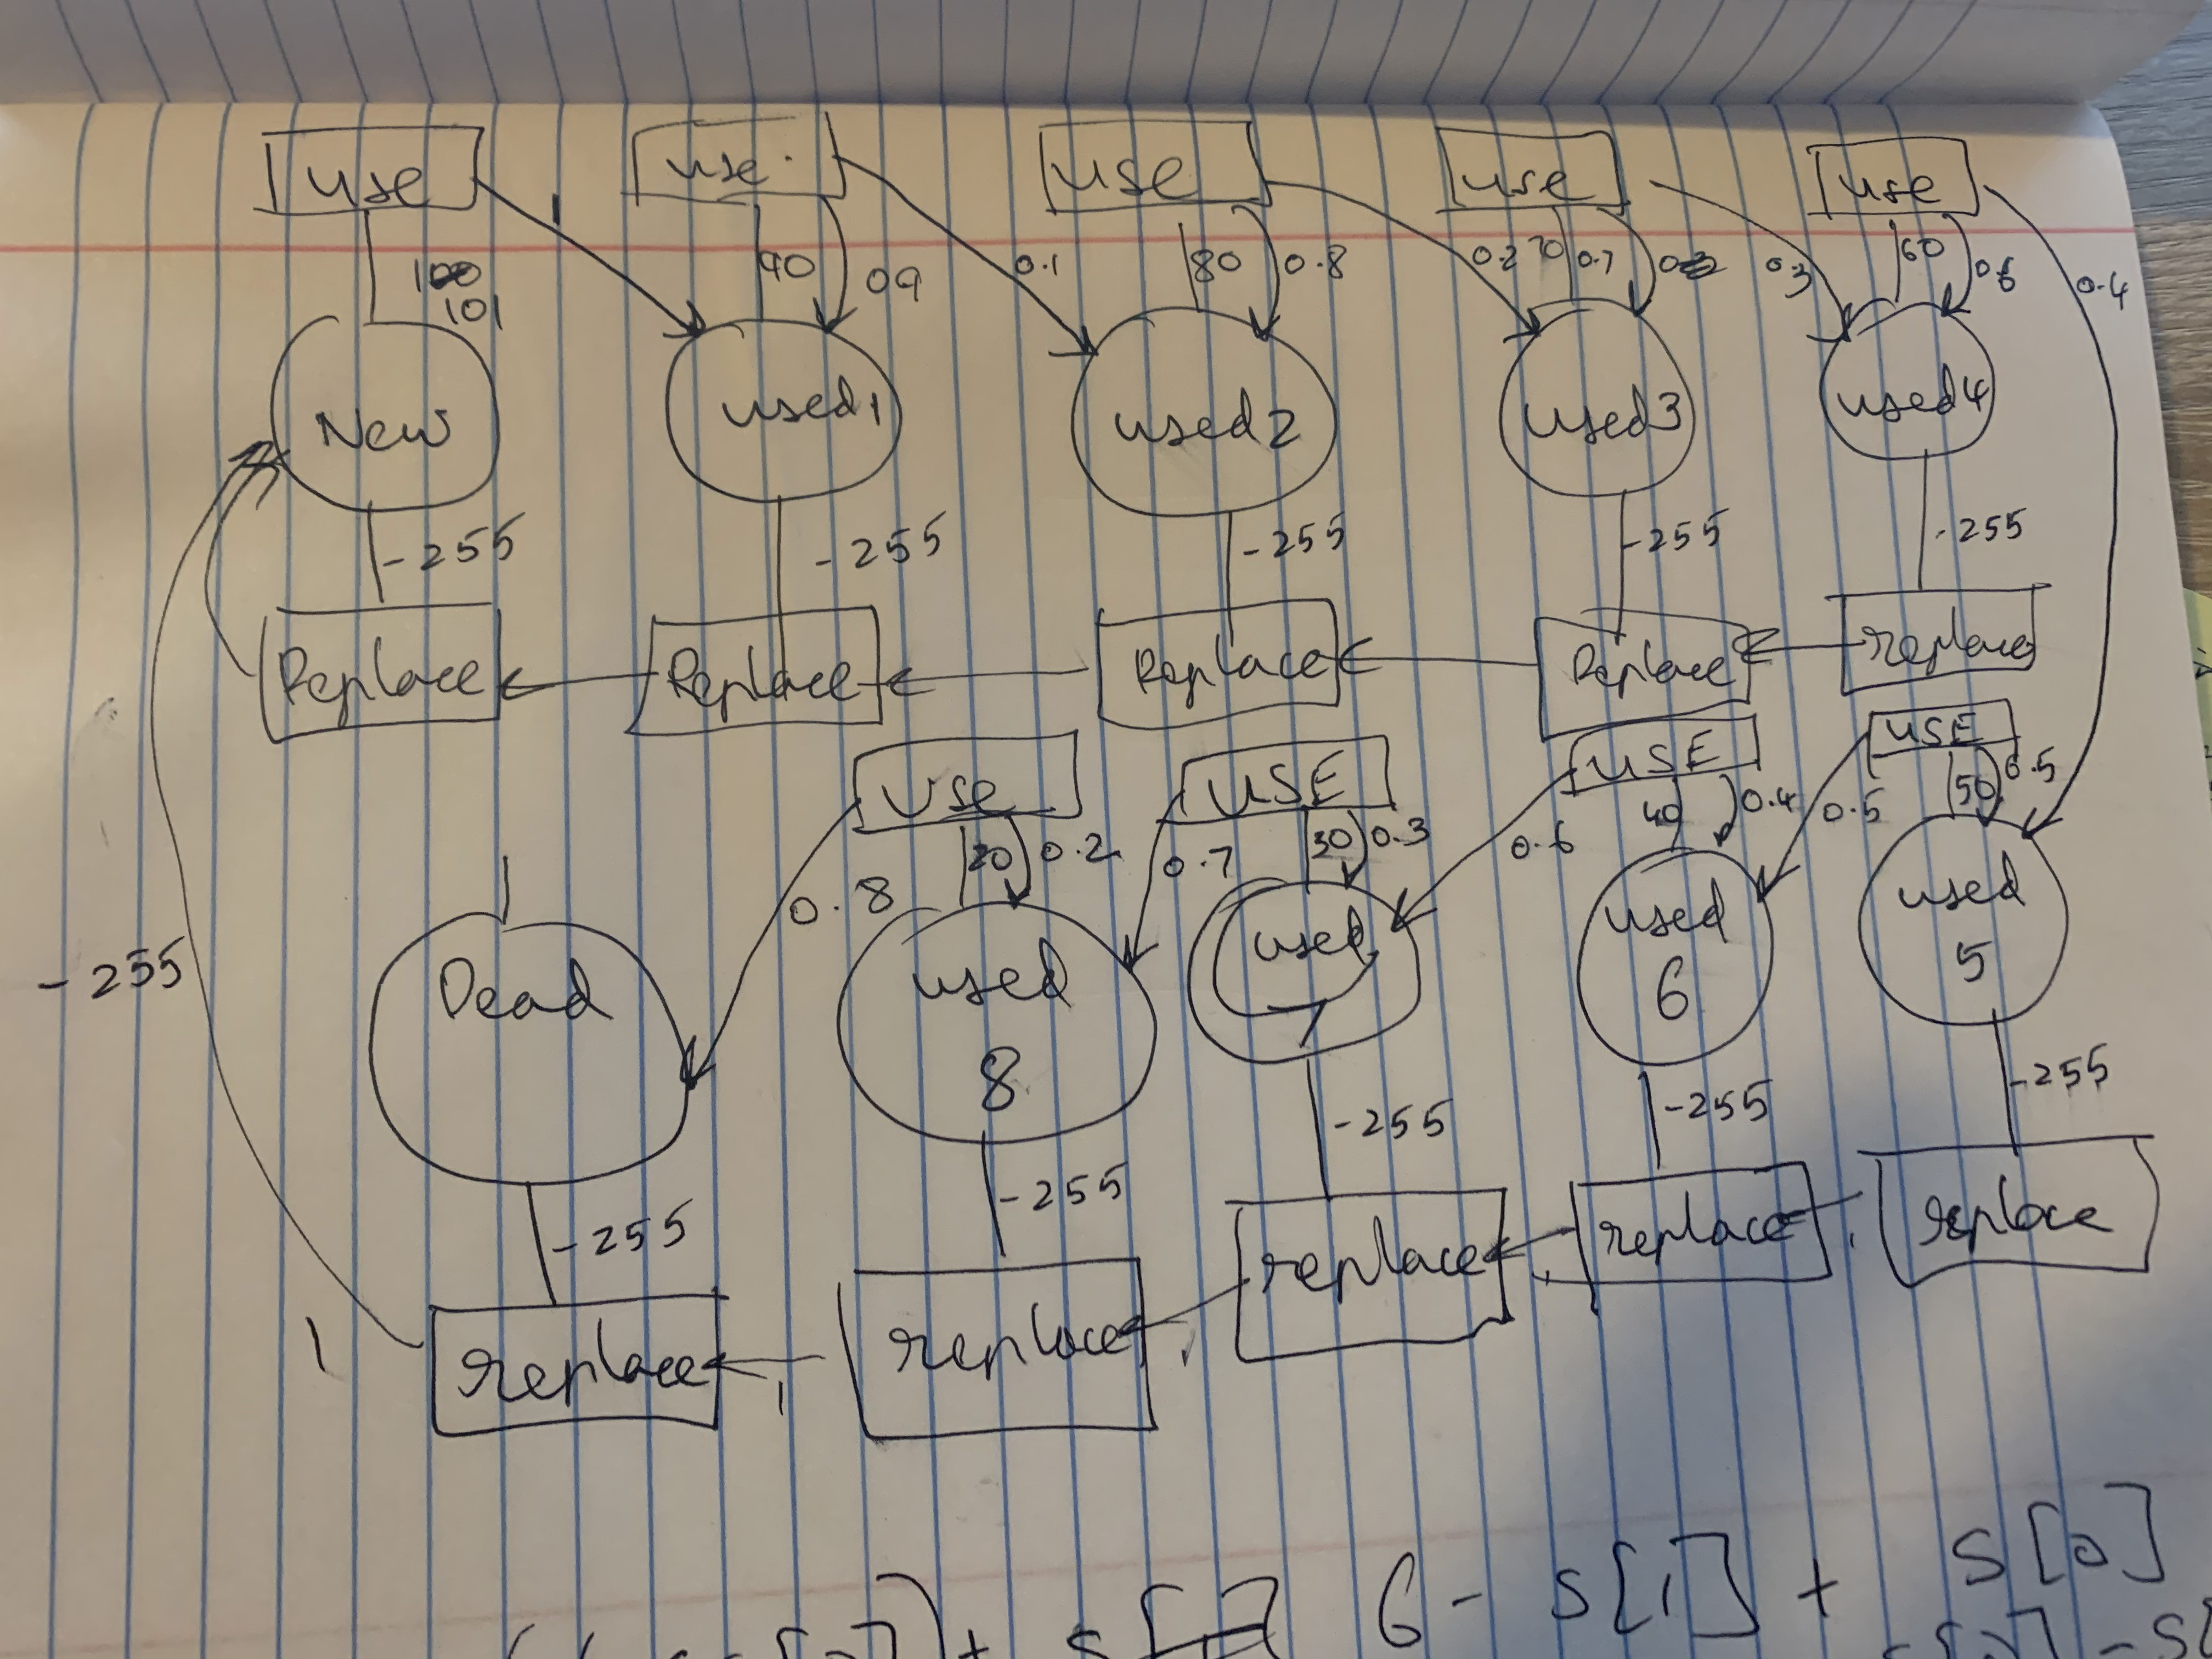
\includegraphics[width=\linewidth]{pls.jpg}
  \caption{State Transition Diagram}
  \label{fig:boat1}
\end{figure}
\subsection{For each of the 10 states, what is the optimal utility (long term expected discounted value) available in that
state (i.e., U \* (state))?}
We use the Bellman's Equation to get the long term expected discounted value available in that state. The utility is simply found by dynamic programming with the following equation.
\begin{center}
$U*(s) = max_{a\in A(s)}[R_{s, a}+\beta (\sum(T_{s, a, s'}U*(s'))]$
\end{center}
Now we get the optimal utility of each state, through brute force, for each state with the following equations. As the question suggests we take the value of $\beta$ as 0.9. To find the optimal utilities we initialize all the utilities to 0 and iterate till there is convergence
\begin{itemize}
\item $U*(NEW) = max[(101+0.9*U*(used1)]$ 
\item $U*(used1) = max[(90+0.9*(0.9*U*(used1)+0.1*U*(used2))), -255+0.9*U*(NEW))]$ 
\item $U*(used2) = max[(80+0.9*(0.8*U*(used2)+0.2*U*(used3))), -255+0.9*U*(NEW))]$ 
\item $U*(used3) = max[(70+0.9*(0.7*U*(used3)+0.3*U*(used4))), -255+0.9*U*(NEW))]$ 
\item $U*(used4) = max[(60+0.9*(0.6*U*(used4)+0.4*U*(used5))), -255+0.9*U*(NEW))]$ 
\item $U*(used5) = max[(50+0.9*(0.5*U*(used5)+0.5*U*(used6))), -255+0.9*U*(NEW))]$ 
\item $U*(used6) = max[(40+0.9*(0.4*U*(used6)+0.6*U*(used7))), -255+0.9*U*(NEW))]$ 
\item $U*(used7) = max[(30+0.9*(0.3*U*(used7)+0.7*U*(used8))), -255+0.9*U*(NEW))]$ 
\item $U*(used8) = max[(20+0.9*(0.2*U*(used8)+0.8*U*(dead))), -255+0.9*U*(NEW))]$ 
\item $U*(dead) = -255 + 0.9*U*(NEW))$ 

\end{itemize}
After training and convergence, these are the utilities that I got:\\
New - 800.8386414296517\\
Used1 - 777.6099848620365\\
Used2 - 641.7355217903227\\
Used3 - 553.8655378421137\\
Used4 - 499.77735155948704\\
Used5 - 471.964104400585\\
Used6 - 465.7547772866866\\
Used7 - 465.7547772866866\\
Used8 - 465.7547772866866\\
Dead - 465.7547772866866\\
We see that after 6 the utilities are the same and thus indicating that the bot decides to replace the machine rather than use it from state used6 onwards. 

\subsection{What is the optimal policy that gives you this optimal utility - i.e., in each state, what is the best action to
take in that state?}
This question can be answered by just looking at the argument/choice/action that gave us the total utility in the above equations. In more formal terms.
\begin{center}
$\pi*(s) = argmax_{a\in A(s)}[R_{s, a}+\beta (\sum(T_{s, a, s'}U*(s'))]$
\end{center}
Where R is the reward, T the transition probability on action a from s to s'.\\
The actions can either be \textbf{USE} or \textbf{REPLACE}.\\ If the first utility function is chosen it is use and if the second utility function is chosen the argmax is replace
\begin{itemize}
\item $\pi*(NEW) = argmax[(101+0.9*U*(used1)]$ 
\item $\pi*(used1) = argmax[(90+0.9*(0.9*U*(used1)+0.1*U*(used2))), -255+0.9*U*(NEW))]$ 
\item $\pi*(used2) = argmax[(80+0.9*(0.8*U*(used2)+0.2*U*(used3))), -255+0.9*U*(NEW))]$ 
\item $\pi*(used3) = argmax[(70+0.9*(0.7*U*(used3)+0.3*U*(used4))), -255+0.9*U*(NEW))]$ 
\item $\pi*(used4) = argmax[(60+0.9*(0.6*U*(used4)+0.4*U*(used5))), -255+0.9*U*(NEW))]$ 
\item $\pi*(used5) = argmax[(50+0.9*(0.5*U*(used5)+0.5*U*(used6))), -255+0.9*U*(NEW))]$ 
\item $\pi*(used6) = argmax[(40+0.9*(0.4*U*(used6)+0.6*U*(used7))), -255+0.9*U*(NEW))]$ 
\item $\pi*(used7) = argmax[(30+0.9*(0.3*U*(used7)+0.7*U*(used8))), -255+0.9*U*(NEW))]$ 
\item $\pi*(used8) = argmax[(20+0.9*(0.2*U*(used8)+0.8*U*(dead))), -255+0.9*U*(NEW))]$ 
\item $\pi*(dead) = argmax(-255 + 0.9*U*(NEW)))$

\end{itemize}
We get that the best policy is as follows\\
State - Policy\\
New - USE\\
used1 - USE\\
used2 - USE\\
used3 - USE\\
used4 - USE\\
used5 - USE\\
used6 - Replace\\
used7 - Replace\\
used8 - Replace\\
Dead  - Replace

\subsection{Instead of buying a new machine, a MachineSellingBot offers you the following option: you could buy a used
machine, which had an equal chance of being in Used 1 and Used 2.
What is the highest price for which this used machine option would be the rational choice? i.e., what price
should MachineSellingBot be selling this option at?}
To calculate this we have to look at the thing it is trying to replace and that is the replace action or "buying a new machine". We can first make an expression for the total discounted utility of buying a used machine. 
\begin{center}
$U*(BuyMachineSellingBot) = -p + 0.9*(0.5*U*(used1)+0.5*U*(used2))$
\end{center}
If we set this equal to the utility function of the replace "button" and get the upperbound of the price. 
\begin{center}
$-p + 0.9*(0.5*U*(used1)+0.5*U*(used2)) = -255 + 0.9*U*(NEW)$
\end{center}
The value of p I get is 173.70\\
We can also verify this empirically. If we set the price of the value above \textbf{173.70} .Above this value, we see that the robot chooses to replace the machine by always buying a new one i.e the utility of buying a new machine is higher, but if we set it to below, the robot always wants to buy a used machine. 

\subsection{For different values of $\beta$ (such that 0 < $\beta$ < 1), the utility or value of being in certain states will change.
However, the optimal policy may not. Compare the optimal policy for $\beta$ = 0.1, 0.3, 0.5, 0.7, 0.9, 0.99, etc. Is there a policy that is optimal for all sufficiently large $\beta$? Does this policy make sense? Explain.}

We can code the following and see what results we get.\\
For $\beta$ = 0.1, 0.3, 0.5, 0.7 this is the policy\\
State - Policy\\
New - USE\\
used1 - USE\\
used2 - USE\\
used3 - USE\\
used4 - USE\\
used5 - USE\\
used6 - USE\\
used7 - USE\\
used8 - USE\\
Dead  - Replace\\
\vspace{2em}\\
For $\beta$ = 0.9, as discussed before \\
State - Policy\\
New - USE\\
used1 - USE\\
used2 - USE\\
used3 - USE\\
used4 - USE\\
used5 - USE\\
used6 - Replace\\
used7 - Replace\\
used8 - Replace\\
Dead  - Replace\\
\vspace{2em}\\
For $\beta$ = 0.99\\
State - Policy\\
New - USE\\
used1 - USE\\
used2 - USE\\
used3 - USE\\
used4 - Replace\\
used5 - Replace\\
used6 - Replace\\
used7 - Replace\\
used8 - Replace\\
Dead  - Replace\\

The policy where you change at used 3 seems to be the policy for all $\beta$ that are sufficiently large. As far as this policy is concerned, this does not make much sense are there is lot of value to be gained states 4 and 5. This policy values the future dollar or the future reward way too much and does not give enough credit to realizing gains at that stage.  
\subsection{Bonus}
The price of the machine in the worst case scenario should give us enough utility so that our robot makes the decision to atleast play the game once. At a certain point the utility to replace is going to get low that the robot is going to start to choose a negative utility. 
\section{Bonus - Dog Picture}
\end{document}